\documentclass[a4paper, 14pt]{extreport}

% ========== MATHEMATICS ==========
\usepackage{amsmath, amssymb}

% ========== MARGINS (GOST R 7.0.97-2025) ==========
\usepackage[
    left=30mm, 
    right=10mm, 
    top=20mm, 
    bottom=20mm,
    headsep=5mm, % Positions page number ~10mm from the top edge
    footskip=10mm
]{geometry}
 \usepackage{graphicx}


\renewcommand{\thefigure}{\thechapter--\arabic{figure}} 
% ========== PARAGRAPHS & SPACING ==========
\usepackage{indentfirst}
\usepackage{setspace}
\onehalfspacing % 1.5 line spacing
\setlength{\parindent}{1.25cm} % Standard GOST indent

% ========== HEADINGS ==========
\usepackage{titlesec}
\titleformat{\chapter}{\normalsize\bfseries\centering}{\thechapter}{1em}{\MakeUppercase}
\titlespacing*{\chapter}{0pt}{-10pt}{20pt}
\titleformat{\section}{\normalsize\bfseries}{\thesection}{1em}{}
\titleformat{\subsection}{\normalsize\bfseries}{\thesubsection}{1em}{}

% ========== PAGE NUMBERING (GOST Style) ==========
\usepackage{fancyhdr}
\pagestyle{fancy}
\fancyhf{}
\fancyhead[C]{\thepage} % Centered at the top
\renewcommand{\headrulewidth}{0pt}

% Apply same style to chapter start pages
\fancypagestyle{plain}{
    \fancyhf{}
    \fancyhead[C]{\thepage}
    \renewcommand{\headrulewidth}{0pt}
}

% ========== TABLES & FIGURES ==========
\usepackage{caption}
\captionsetup[table]{labelsep=endash, justification=raggedright, singlelinecheck=off}
\captionsetup[figure]{labelsep=endash, justification=centering}

% ========== BIBLIOGRAPHY ==========
\usepackage[
    backend=biber,
    style=gost-numeric,
    sorting=none
]{biblatex}
\addbibresource{bibliography.bib}

% ========== HELPER PACKETS ==========
\usepackage{enumitem}
\setlist{nosep, leftmargin=\parindent}
\usepackage[unicode, hidelinks]{hyperref}
\usepackage[T2A]{fontenc}
\usepackage[utf8]{inputenc}
\usepackage[russian, english]{babel}
% ========== DOCUMENT START ==========
\begin{document}

% ========== TITLE PAGE (GOST R 7.0.97-2025 COMPLIANT) ==========
\begin{titlepage}
	\centering
	{MINISTRY OF SCIENCE AND HIGHER EDUCATION OF THE RUSSIAN FEDERATION \par}
	{\normalsize Federal State Budgetary Educational Institution of Higher Education \par}
	{"CHELYABINSK STATE UNIVERSITY" \par}
	(CSU) \par
	\vspace{5pt}
	{\normalsize Institute of Information Technology \par}

	\vspace{80pt}

	{\large THESIS \par}
	\vspace{20pt}

	{\Large Development of the University Navigator architecture \par}

	\vspace{60pt}

	\begin{flushright}
		\begin{minipage}{0.45\textwidth}
			{\bfseries Authors:} \\
			Chikishev Mikhail, PR-102\\
			Mikhail Sharmanov, PR-103\\
			Andreev Alexey, PR-103\\
			Egor Yemelyanov, PR-103
		\end{minipage}
	\end{flushright}

	\vfill

	{\normalsize Chelyabinsk \par}
	{\normalsize 2026 \par}
\end{titlepage}

\setcounter{page}{2}
\tableofcontents
\chapter{Introduction}
\section{Thesis Rationale}
The thesis aims to design backend architecture for a replacement of existing navigation service \href{https://map.csu.ru}{map.csu.ru}. The primary driver for the thesis is the need to implement modern 360-degree panoramic imaging technologies to enhance the visualization of the university environment. During the conceptual discussion, it was decided to discontinue support for the current codebase in favor of designing and developing a fundamentally new application. This decision is based on the following factors:
\begin{enumerate}
	\item low cost-effectiveness of maintaining the previous version due to accumulated technical debt and architectural complexity;
	\item the necessity of implementing a modern technology stack to ensure scalability and performance.
\end{enumerate}

The thesis objective is to design a backend of multifunctional ecosystem that addresses key university digitalization challenges and improves the Quality of Life (QoL) for students and staff. 

\section{Object and subject}

The subject of the thesis is the active team communication, the study of materials required for the development of the backend architecture, the analysis of existing technical solutions, and the collective decision-making process undertaken during the system design.

The object of the thesis is the set of application and backend flowcharts, along with the description of their interaction.

\chapter{Theoretical Framework}

\section{Analysis of Current Challenges}
The academic process is currently associated with several organizational complexities. These include the absence of a unified secure environment for real-time communication between students and faculty, the decentralization of university information resources, and the low efficiency of notification channels.

The architecture of the project under development is designed to aggregate the necessary services within a single interface, thereby enhancing the transparency and accessibility of the educational environment.

\subsection{Survey Results}
To validate these assumptions, a preliminary survey was conducted among students. A total of 19 respondents participated, with 8 responses collected via Google Forms (the data below reflect this subset; the remaining 11 responses came from other channels and showed a similar distribution).

The key questions and answers for are summarised as follows:

\begin{itemize}
    \item \textbf{Navigation within the university:}  
    7 out of 8 respondents (87.5\%) reported experiencing difficulties. Only 1 respondent (12.5\%) answered ``No''.
    \item \textbf{Academic communication:}  
    7 out of 8 (87.5\%) face problems with study‑related communication. 1 respondent (12.5\%) does not experience such issues.
    \item \textbf{Accessing the schedule:}  
    5 out of 8 (62.5\%) find it problematic to obtain the current schedule, while 3 respondents (37.5\%) answered ``No''.
\end{itemize}

These results confirm that the majority of students encounter obstacles in all three areas. In particular, navigation and communication problems are nearly universal (87.5\% each), while schedule access, though somewhat less critical, still affects almost two‑thirds of the respondents. The data strongly support the need for an integrated navigator that addresses wayfinding, messaging, and timetable delivery within a single environment.

\section{Tasks}

\subsection{Theoretical Tasks (Subject of the Research)}
\begin{itemize}
	\item facilitate active team communication to discuss the desired system functionalities;
	\item conduct a collaborative analysis and discuss possible methods for implementing each functionality;
	\item review the scientific and technical materials required for designing the backend architecture.
\end{itemize}

\subsection{Practical Tasks (Object of the Research)}
\begin{itemize}
	\item develop a high-level application flowchart illustrating the interaction among all modules;
	\item create a detailed backend flowchart.
\end{itemize}
\section{Study of Technical Materials for Backend Architecture Design}

As part of the theoretical subject of this thesis, a systematic study of technical materials was conducted to inform the creation of the application and backend flowcharts (the object of the research). The study covered four essential areas.

First, the Go programming language was examined using official documentation~\cite{go.dev}, the MetaNIT tutorials~\cite{metanit.go, metanit.web}, and a Stepik course~\cite{stepik.go}. These sources provided foundational knowledge of Go's concurrency model, web programming capabilities, and microservices design patterns.

Second, geospatial routing technologies were investigated, focusing on pgRouting~\cite{pgrouting.docs} and its integration with PostgreSQL, as well as practical implementations using OpenStreetMap data. Articles from Habr~\cite{habr.pgrouting} provided real-world insights into building routing systems.

Third, supporting infrastructure components were reviewed, including Redis for caching and queuing, Asynq~\cite{asynq} for distributed task processing, and MinIO for object storage of panoramic images. Key Habr resources~\cite{habr.redis, habr.minio, habr.asynq} guided these decisions.

Fourth, security practices were studied, specifically the "Shift Left Security" paradigm and its application to Go microservices.

The synthesis of these materials directly shaped the architectural decisions documented in the application and backend flowcharts, thereby completing the theoretical subject of the thesis.
\section{Core Development Principles}
The key priorities in system design are security, performance, portability, and maintainability. These requirements dictated the choice of the technology stack. Several languages, including Python, JavaScript, and C\#, were excluded from consideration as they did not meet the performance criteria or the specific architectural requirements of the thesis.

Furthermore, a significant objective for the project team is to gain hands-on experience with high-performance systems and to master industry-relevant skills.


\section{Panoramic Content Visualization Methods}
To achieve a full sense of presence and indoor navigation, 360-degree panoramic imaging technologies will be employed. The key task in the software processing of such content will be the transformation of spherical data into a flat image and its subsequent re-projection within the user interface.

The primary standard used will be the equirectangular projection, where the coordinates of each point on the sphere will be mapped to the Cartesian coordinates of the image pixels.

Within the scope of this thesis, 360-degree map visualization will be implemented using the specialized rendering library \texttt{three.js}, which will map the equirectangular texture onto the inner surface of a virtual sphere or cube. To optimize client-side performance, a segmented loading (tiling) technique will be applied, avoiding excessive RAM consumption when handling ultra-high-resolution images.

\section{Routing Fundamentals}
The system will be based on a mathematical model of a weighted directed graph, constructed according to the principle of Poincaré duality. In this model, 3D indoor volumes will be transformed into nodes, while the connecting surfaces will become edges. The integration of the IndoorGML standard will allow for dynamic network filtering via the \texttt{pgRouting} extension. This will enable the calculation of the shortest path using Dijkstra's algorithm on an up-to-date subgraph that accounts for the physical connectivity of floors in real-time.

\section{Distributed Communication Protocols}
To establish a unified interaction environment, the XMPP (Extensible Messaging and Presence Protocol) will be selected. Unlike proprietary solutions, XMPP is based on open XML standards and provides high extensibility through XEP specifications.

The choice of the \texttt{ejabberd} server is driven by its fault tolerance, robust API, and ability to handle a large number of concurrent connections. In the application architecture, \texttt{ejabberd} will serve as a module providing:
\begin{itemize}
	\item real-time instant messaging;
	\item isolation of personal social networks from the learning process;
	\item multi-user conference management for organizing study groups;
	\item user notification services.
\end{itemize}
The protocol integration will ensure a communication channel decoupled from personal data, maintaining traffic and message encryption.

\section{Information Security}
Data protection will be addressed at all stages of the Software Development Life Cycle (SDLC). The choice of the Go programming language is justified by its safety mechanisms (like in KISS). To minimize attack vectors, the following solutions will be implemented:
\begin{itemize}
	\item use of ORM to prevent SQL injections;
	\item application of Anubis for protection against automated attacks (bots);
	\item implementation of specialized Middleware;
	\item use of JWT for user authorization;
	\item deployment in "distroless" containers to reduce the attack surface;
	\item integration of static analyzers and Quality Gates into the CI/CD process.
\end{itemize}
This approach will implement the "Shift Left Security" concept, allowing for the identification and remediation of vulnerabilities at the early stages of the development cycle.

\chapter{Practical Implementation}
\section{General Architecture Overview}
\begin{figure}[h]
	\centering
	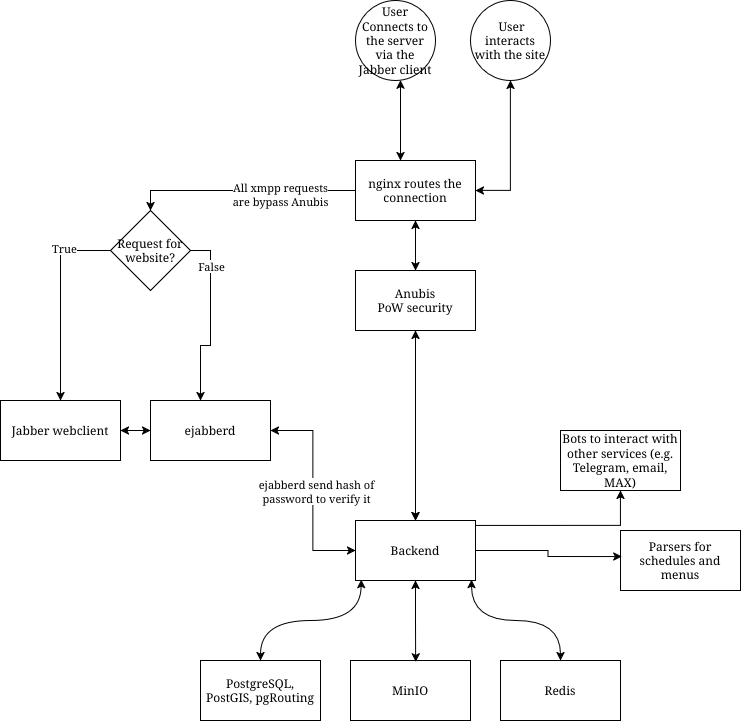
\includegraphics[width=\textwidth, height=0.9\textheight, keepaspectratio]{images/Overview.drawio.png}
	\caption{Proposed architecture diagram}
	\label{fig:overview}
\end{figure}
The general architecture to be developed is presented in Fig. \ref{fig:overview}.
The designed system architecture is dictated by the specifics of the target infrastructure — deployment within an isolated virtual machine (VM) with limited computing resources. These conditions impose several constraints on the use of orchestration tools and necessitate a transition to a hybrid software development model.

\subsection{Infrastructure Characteristics and Design Principles}
The choice of a \texttt{docker-compose} based deployment environment limits horizontal scaling capabilities in the short term; however, it ensures high autonomy in system resource managment. The core architectural principles will include:
\begin{itemize}
	\item {Service Consolidation:} Minimizing the number of containers to reduce virtualization overhead.
	\item {Hybrid Monolith:} Business logic will be implemented within a single service (Backend) to simplify inter-node communication.
	\item {Stateless Approach:} The backend will be designed without session state persistence, ensuring readiness for future scaling via Kubernetes.
\end{itemize}

\subsection{Technology Stack Components}
\begin{enumerate}
	\item Networking and Security (NGINX, Anubis) \\
	      To handle traffic routing and ensure security, a combination of NGINX and the Anubis protection system will be utilized. This solution will be critical for preventing system performance degradation caused by unauthorized traffic spikes.

	\item Storage and Geospatial Analysis Layer (PostgreSQL, PostGIS, pgRouting) \\
	      PostgreSQL will be used as the primary DBMS. The PostGIS extension will provide efficient storage of spatial data, while the pgRouting extension will be integrated to execute shortest-path algorithms directly on the database side.

	\item Communication Subsystem (Ejabberd and XMPP Client) \\
	      The \texttt{ejabberd} server will be used to facilitate user interaction. User authentication will be delegated to the main backend using the OAuth protocol to enable a Single Sign-On (SSO) concept.

	\item Object Storage and Caching (MinIO, Redis) \\
	      Static content will be stored in the \texttt{MinIO} object storage. \texttt{Redis} will be employed for task queue management and real-time data caching to improve system response times.

	\item External Integration Services (Parsers and Bots) \\
	      Data collection modules will be implemented in Python for flexibility. For chat-bot development, priority will be given to the Go language to minimize resource consumption.
\end{enumerate}
\section{Backend Implementation}
The backend of the application will be developed in Go using a multi-layered architecture. This section examines the application lifecycle and subsystems based on the plan shown in Fig. \ref{fig:backend}.

\begin{figure}[h]
	\centering
	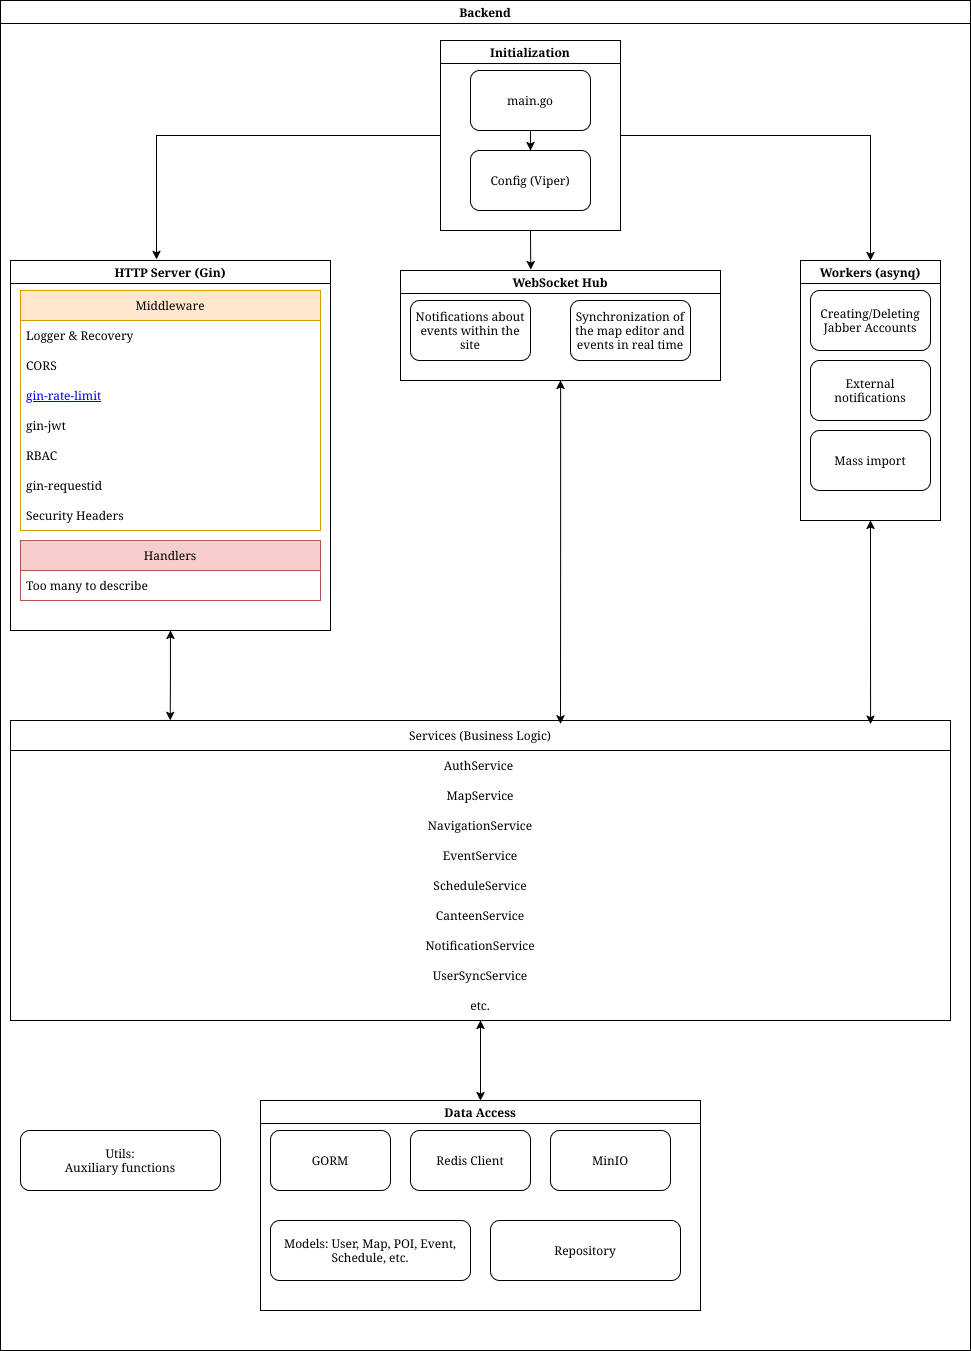
\includegraphics[width=\textwidth, height=0.9\textheight, keepaspectratio]{images/Backend.png}
	\caption{Planned backend block diagram}
	\label{fig:backend}
\end{figure}

\subsection{Component Initialization and Deployment Process}
The application startup will follow a strictly deterministic sequence. The deployment algorithm will include:
\begin{enumerate}
	\item {Configuration:} Using \texttt{Viper} to load environment parameters for flexible setting adjustments.
	\item {Database State Management:} Executing automatic migrations using \texttt{golang-migrate} to guarantee data schema consistency.
	\item {Caching and Queue Initialization:} Creating clients for \texttt{Redis} and \texttt{Asynq}.
	\item {Dependency Injection (DI):} Implementing the IoC (Inversion of Control) pattern to facilitate unit testing and eliminate hidden dependencies.
	\item {Transport Layer Startup:} Initializing HTTP server routes and activating background workers.
\end{enumerate}

\subsection{Transport Layer and Request Processing}
The \texttt{Gin} framework was selected as the primary HTTP framework. The lifecycle of an incoming request will include passing through a chain of \textit{middleware}, routing to the handler, and invoking business logic via the service layer. To ensure interactivity, a {WebSocket Hub} subsystem will be implemented.

\subsection{Abstraction Layers: Services and Repositories}
The application architecture is divided into logical levels to isolate business logic from infrastructure implenation details:
\begin{enumerate}
	\item {Service Layer:} Will encapsulate the core business logic of the application. Services will operate with DBMS through repository interfaces, remaining independent of specific storage implementations.
	\item {Data Access Layer (DAL):} Will be implemented via the "Repository" pattern to hide the details of SQL queries.
	\item {Interface Abstraction:} The use of interfaces will allow for the replacement of real database connections with \textit{mock} objects during testing.
\end{enumerate}

\subsection{Background Tasks and Asynchronous Processing}
The \texttt{Asynq} library will be used to perform resource-intensive operations, such as schedule parsing. Tasks will be placed into a \texttt{Redis} queue and processed by dedicated workers to keep the main HTTP server responsive.

\section{DevOps Methodology and Information Security}
A modern CI/CD cycle centered on the "Shift Left Security" concept will be implemented within the thesis. The primary objective will be to identify defects at the earliest possible stages.

\subsection{Continuous Integration (CI) Pipeline and Quality Assurance}
The code build and verification process will be automated using the {Jenkins} automation server. The lifecycle of changes will include:
\begin{enumerate}
	\item {Automated Testing:} Every Pull Request will trigger a suite of unit and integration tests.
	\item {Static Analysis and Quality Gates:} Source code will undergo scanning in {SonarQube} to assess technical debt and vulnerabilities.
	\item {Mandatory Code Review:} Branch merging will be permitted only upon approval from other members of the development team.
\end{enumerate}

\subsection{Containerization and Runtime Security}
To minimize attack vectors, containerization technology utilizing specialized images will be employed.
\begin{itemize}
	\item {Distroless Containers:} The application will use \textit{distroless} images to reduce the "attack surface" by excluding unnecessary OS utilities.
	\item {Multi-stage Builds:} The Go application will be compiled in an intermediate container to ensure a minimalist final image.
\end{itemize}

\chapter{Conclusion}

In accordance with the research tasks defined in this thesis, the work was structured around two complementary dimensions: the subject and the object.

Regarding the subject of the thesis, all theoretical tasks were successfully completed. Active team communication was facilitated to discuss the desired system functionalities. Collaborative analysis was conducted to evaluate possible implementation methods for each function. Furthermore, the necessary scientific and technical materials required for designing the backend architecture were thoroughly studied.

Regarding the object of the thesis, the practical tasks were fulfilled as follows. A high-level application flowchart illustrating the interaction among all modules was developed. In addition, a detailed backend flowchart, including data flow descriptions and request processing logic, was created. These flowcharts collectively document the proposed architecture of a multifunctional university navigation ecosystem.

The key expected outcomes of the thesis, as reflected in its object, include:
\begin{itemize}
	\item \textbf{Architectural Modernisation:} The designed modular structure, formalised in the flowcharts, provides a foundation for replacing outdated visualisation tools and establishing a unified digital space.
	\item \textbf{Navigation Innovation:} The detailed backend flowchart incorporates provisions for accurate indoor routing (e.g., via integration with frameworks such as pgRouting), while the application flowchart includes support for 360-degree panoramas as a visual aid.
	\item \textbf{Security and Reliability:} The architectural design follows the principles of the "Shift Left Security" concept, and the documented component separation enables the use of minimal (e.g., distroless) containers for deployment.
	\item \textbf{Scalability:} The technology stack indicated in the technical specification (derived from the object of this thesis) allows for seamless project scaling as load increases.
\end{itemize}

Once implemented based on the designed flowcharts, the system will comply with modern standards and provide a significant improvement in the quality of interaction within the university's digital environment. Thus, the theoretical subject (team processes and study) enabled the creation of the practical object (application and backend flowcharts), which in turn fully addresses the initial challenges.
\begin{thebibliography}{9}
\bibitem{go.dev} Go Authors. (n.d.). \textit{Go Documentation}. \url{https://go.dev/doc/}

\bibitem{metanit.go} MetaNit. (n.d.). \textit{Руководство по языку Go}. \url{https://metanit.com/go/tutorial/}

\bibitem{metanit.web} MetaNit. (n.d.). \textit{Руководство по веб-программированию языку Go}. \url{https://metanit.com/go/web/}

\bibitem{stepik.go} Stepik. (n.d.). \textit{Course: Development of Web Services in Golang}. \url{https://stepik.org/course/187490/promo}

\bibitem{pgrouting.docs} pgRouting Contributors. (n.d.). \textit{pgRouting Documentation (latest)}. \url{https://docs.pgrouting.org/latest/en/index.html}

\bibitem{habr.pgrouting} Habr. (2019). \textit{Делаем маршрутизацию (роутинг) на OpenStreetMap. Введение}. \url{https://habr.com/ru/articles/511144/}

\bibitem{habr.redis} ManyChat. (2020). \textit{Redis на практических примерах}. \url{https://habr.com/ru/companies/manychat/articles/507136/}

\bibitem{habr.minio} OzonTech. (2021). \textit{Зачем и как хранить объекты на примере MinIO}. \url{https://habr.com/ru/companies/ozontech/articles/586024/}

\bibitem{asynq} Hibiken. (n.d.). \textit{Asynq}. \url{https://github.com/hibiken/asynq}

\bibitem{habr.asynq} Wunderfund. (2021). \textit{Разбираемся с Redis}. \url{https://habr.com/ru/companies/wunderfund/articles/685894/}

\end{thebibliography}
\end{document}
